\chapter{Implementation and Results}\label{cha:implementation}

\section{Front-end}\label{cha:implementation:sec:front-end}

\subsection{Component Structure}
When developing the Angular front-end over the \texttt{Sb-Admin-Material} template, it was noted that the example pages that could be accessed by links listed in the left sidebar, seen on Figure~\ref{fig:visible}, were found inside the \texttt{/app/layout} folder. Therefore it made sense to follow this approach and implement \gls{Yabi}'s custom pages in the same place.

In general, each entity have got a folder that contains:
\begin{itemize}
\item A ``model'' file with:
  \begin{itemize}
  \item A class that represents the entity, to be used when retrieving entities depending on the current user.
  \item A class that extends \texttt{PagingAndSortingRepository}, to map Spring Repository responses.
  \item A class that extends \texttt{Entity}, representing the elements contained within the repository response.
  \item A repository ``accessor'' that indicates key used to access the list of \texttt{Entity} contained within the repository response.
  \end{itemize}
\item A Service file that extends \texttt{PagingAndSortingRepository}, specifying it for the given entity.
\item The Module file declaring its dialog Components to also be loaded.
\item The Template file that renders a listing with the available entities.
\item The Component file that interacts with the Template.
\item The Style file with rules to correctly render the ``add'' button.
\item A folder with a dialog Component for creating more entries.
\item A folder with a dialog Component for editing an entry.
\end{itemize}

There are some variations to this rule. \texttt{User} Component only has only one dialog that is used to show more information about the current user. \texttt{Query} Component was one of the first components to be developed and it has three dialogs, one for showing more information and the results of running it, one for creating new queries that is not used and a ``form'' dialog that maps a \texttt{Query} to input elements that is used for editing and creating.

\subsubsection{Components \& Dialogs}

\todo{\texttt{LoginComponent}}

directory
\begin{figure}
  \centering
  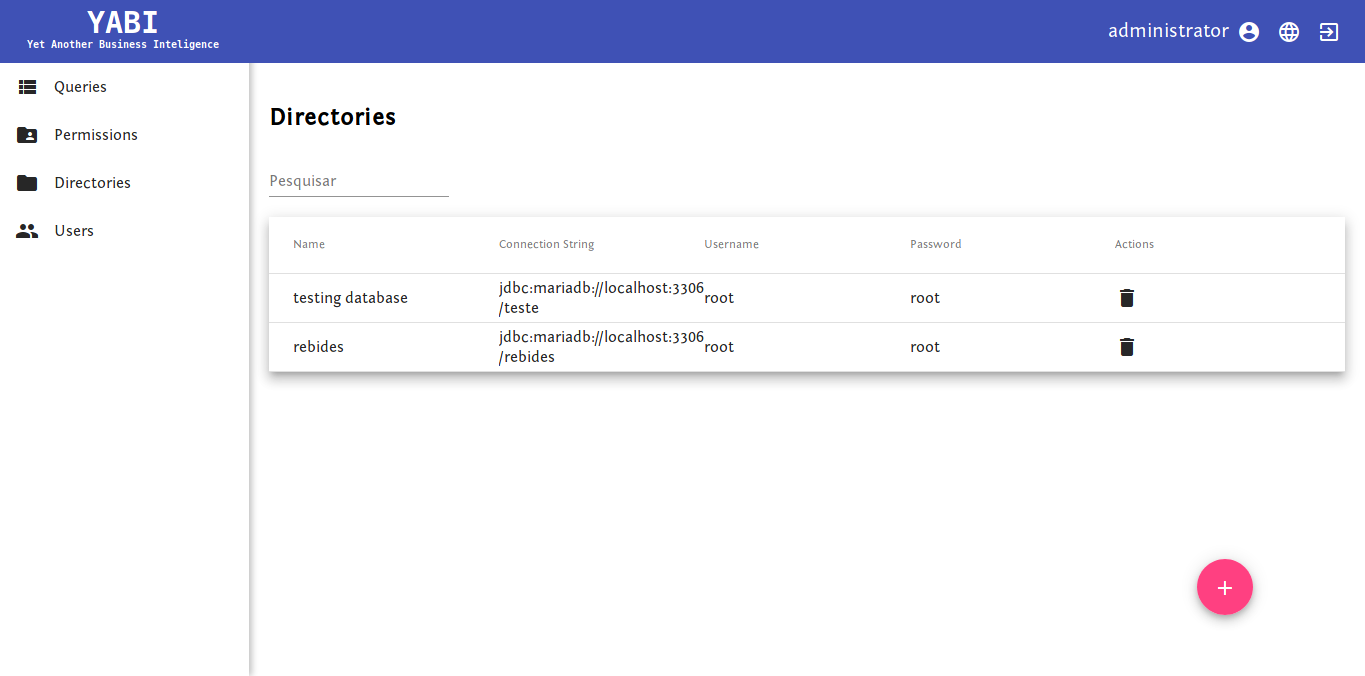
\includegraphics[width=.8\textwidth]{images/screenshots/directory/directory-listing}
  \caption{Listing of all registered \texttt{Directory}}\label{fig:dirlist}
\end{figure}

\begin{figure}
  \centering
  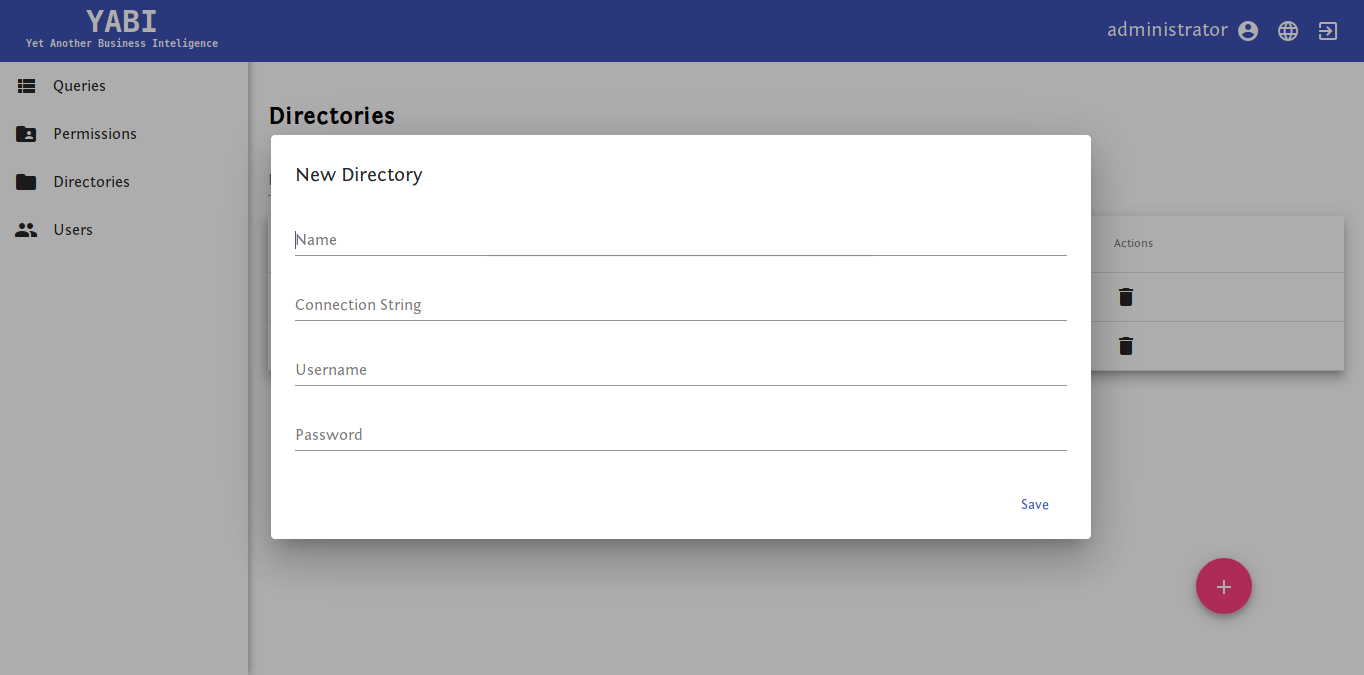
\includegraphics[width=.8\textwidth]{images/screenshots/directory/directory-new}
  \caption{Dialog for creating a new \texttt{Directory}}\label{fig:dirnew}
\end{figure}

\begin{figure}
  \centering
  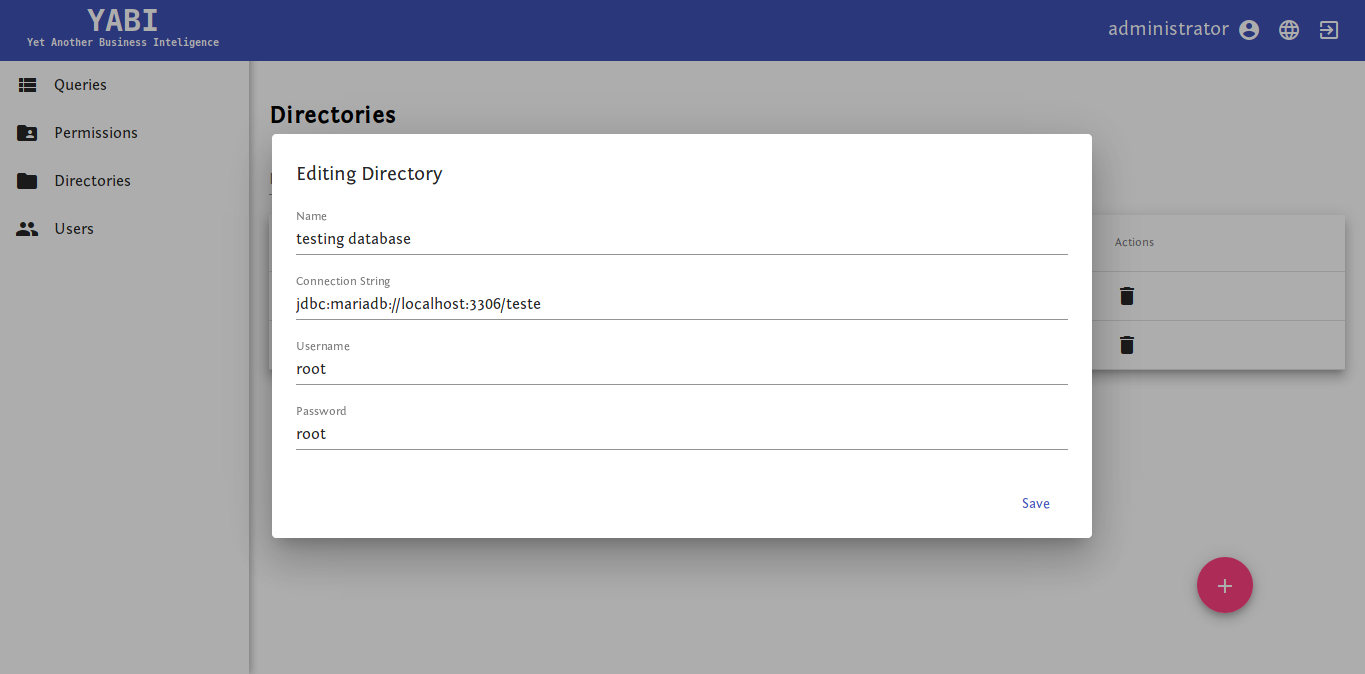
\includegraphics[width=.8\textwidth]{images/screenshots/directory/directory-edit}
  \caption{Dialog for editing an existing \texttt{Directory}}\label{fig:diredit}
\end{figure}

query
\begin{figure}
  \centering
  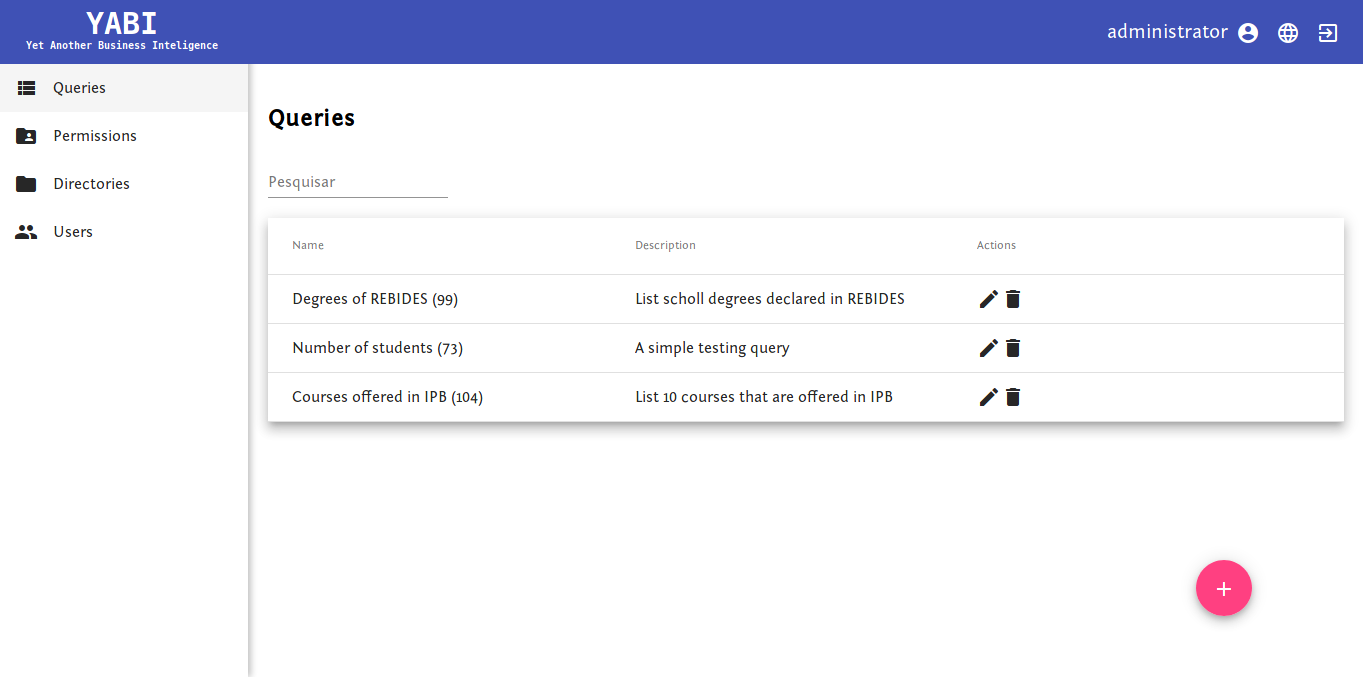
\includegraphics[width=.8\textwidth]{images/screenshots/query/query-listing}
  \caption{Listing of all registered \texttt{Query}}\label{fig:querylist}
\end{figure}

\begin{figure}
  \centering
  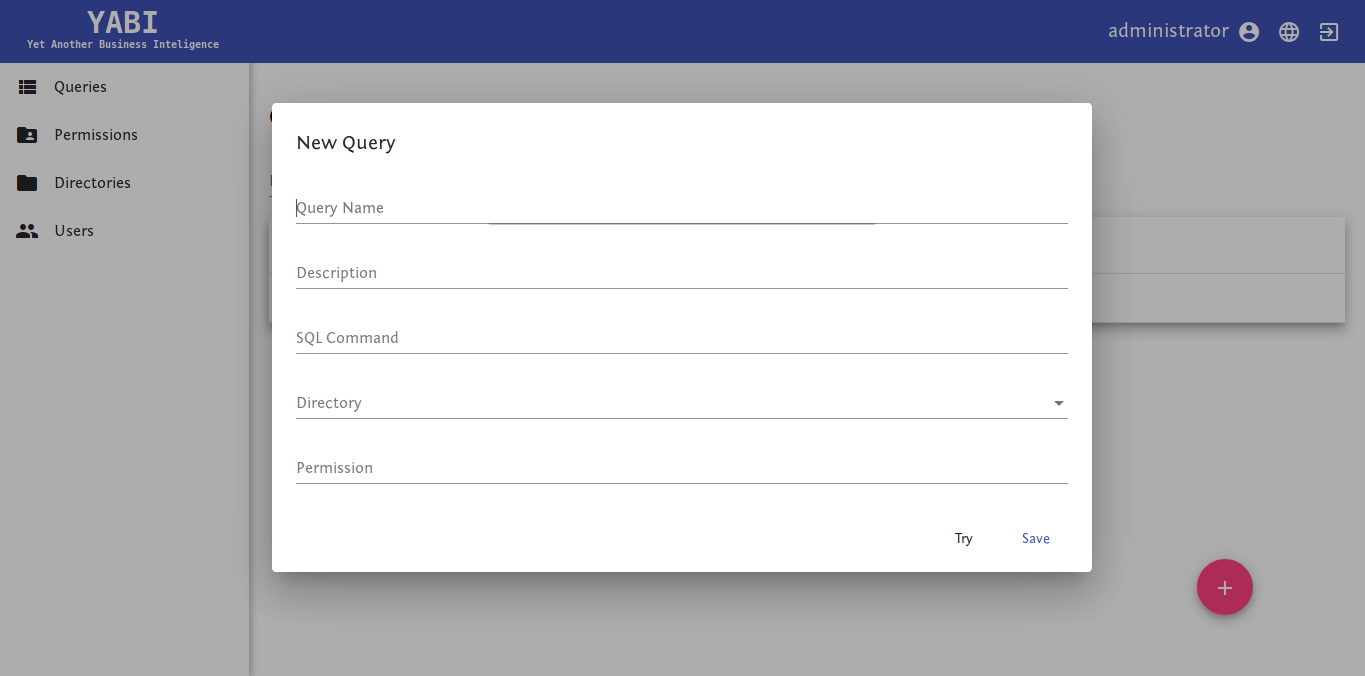
\includegraphics[width=.8\textwidth]{images/screenshots/query/query-new}
  \caption{Dialog for creating a new \texttt{Query}}\label{fig:querynew}
\end{figure}

\begin{figure}
  \centering
  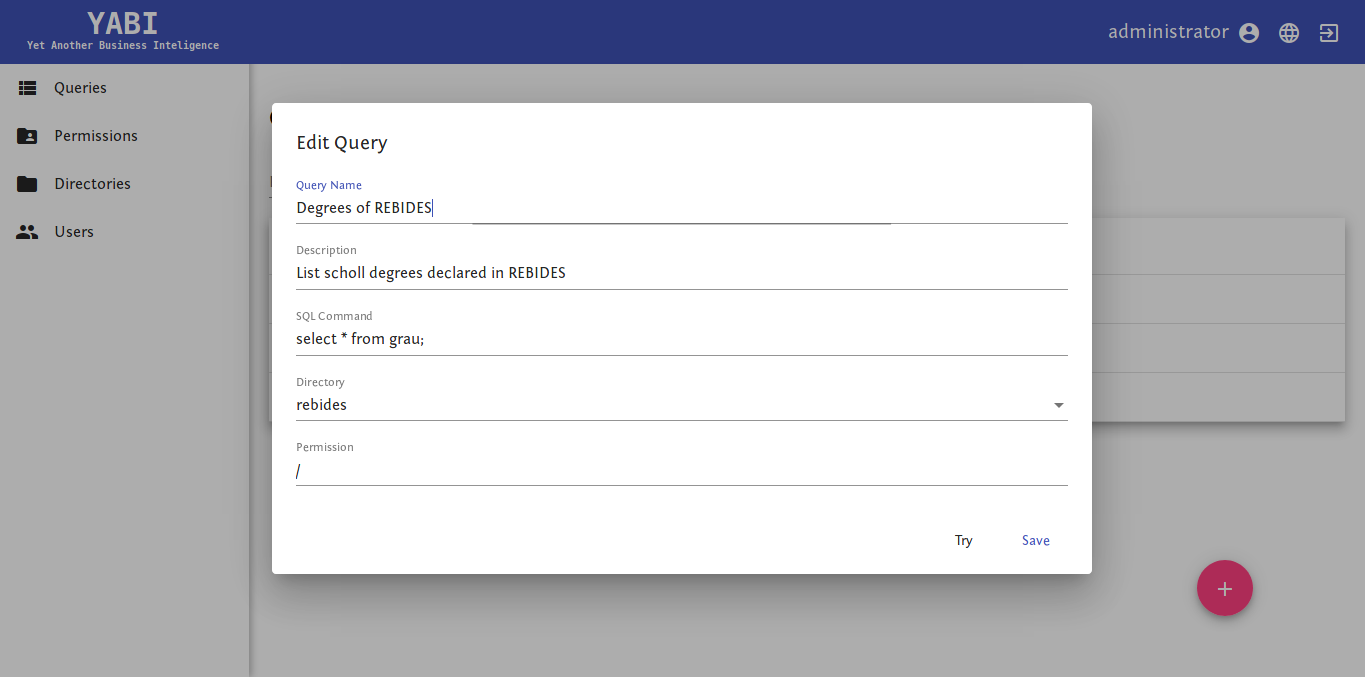
\includegraphics[width=.8\textwidth]{images/screenshots/query/query-edit}
  \caption{Dialog for editing an existing \texttt{Query}}\label{fig:queryedit}
\end{figure}

\begin{figure}
  \centering
  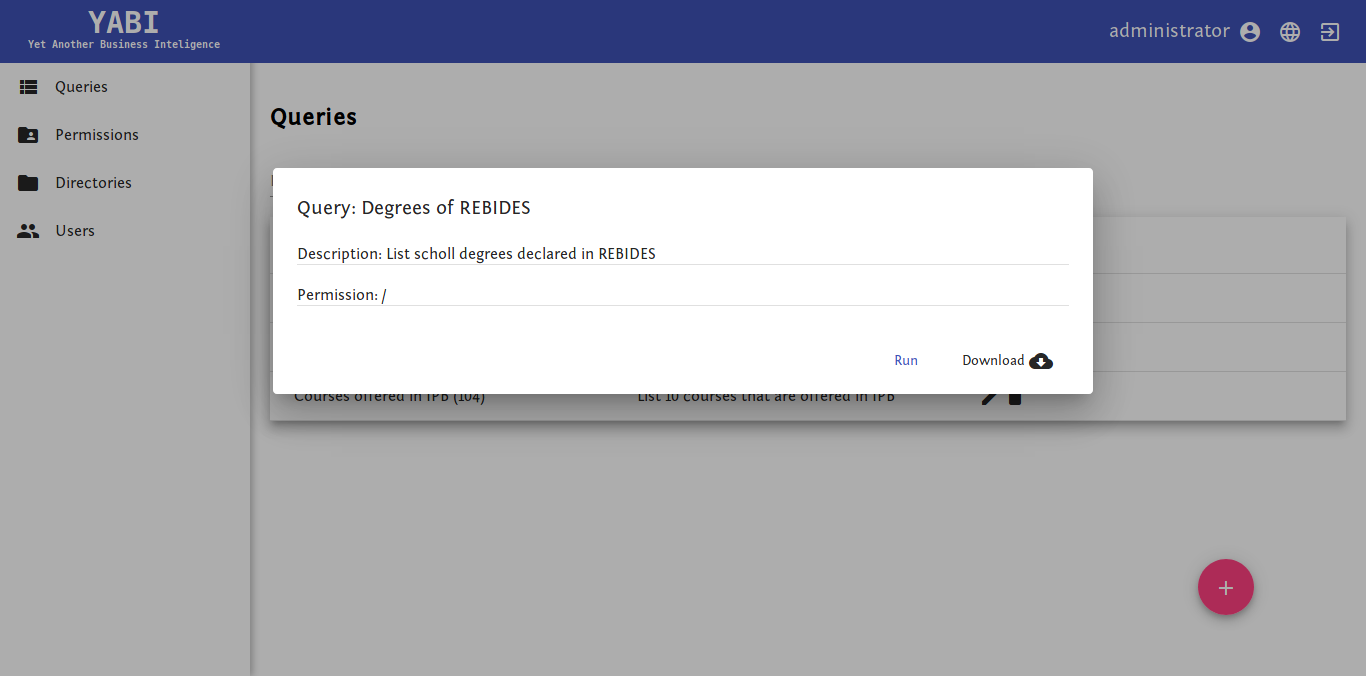
\includegraphics[width=.8\textwidth]{images/screenshots/query/query-pre-run}
  \caption{Dialog for running a \texttt{Query}}\label{fig:queryprerun}
\end{figure}

\begin{figure}
  \centering
  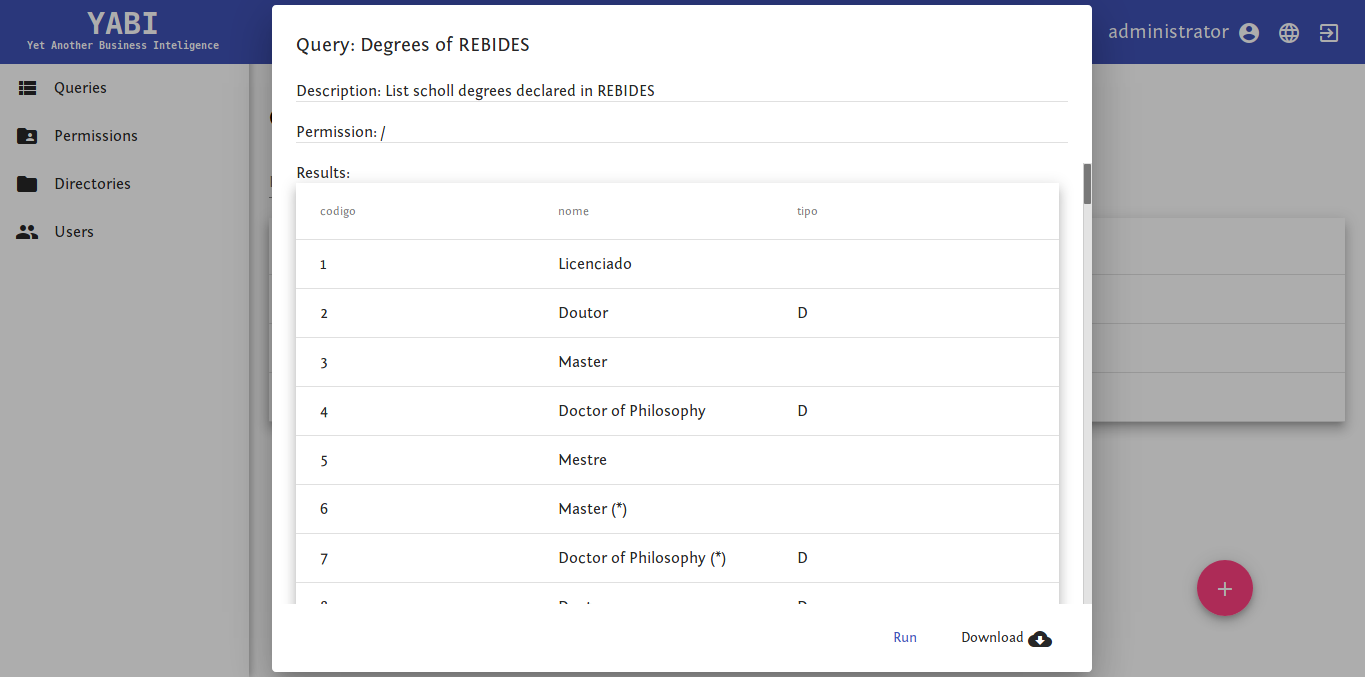
\includegraphics[width=.8\textwidth]{images/screenshots/query/query-post-run}
  \caption{Dialog for running a \texttt{Query} after it was executed}\label{fig:querypostrun}
\end{figure}

permission

\begin{figure}
  \centering
  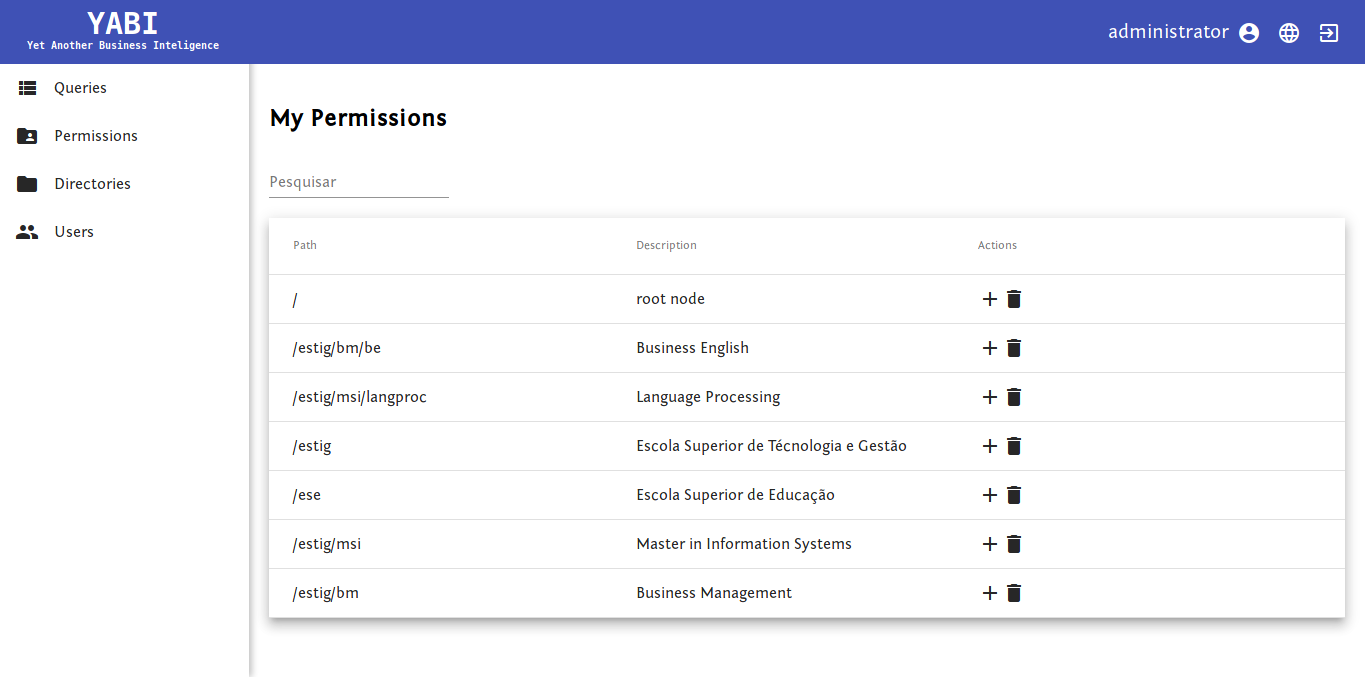
\includegraphics[width=.8\textwidth]{images/screenshots/permission/permission-listing}
  \caption{Listing of all registered \texttt{Permission}}\label{fig:permissionlist}
\end{figure}

\begin{figure}
  \centering
  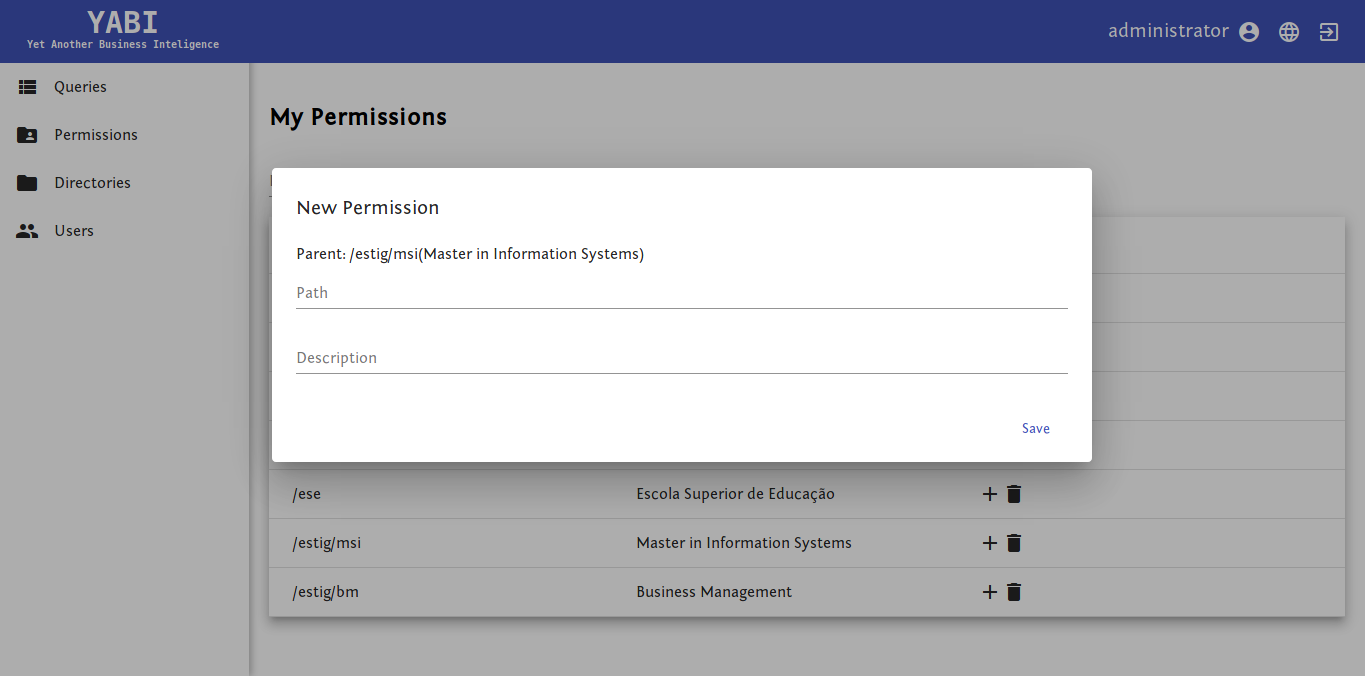
\includegraphics[width=.8\textwidth]{images/screenshots/permission/permission-new}
  \caption{Dialog for creating a new \texttt{Permission}}\label{fig:permissionnew}
\end{figure}

\begin{figure}
  \centering
  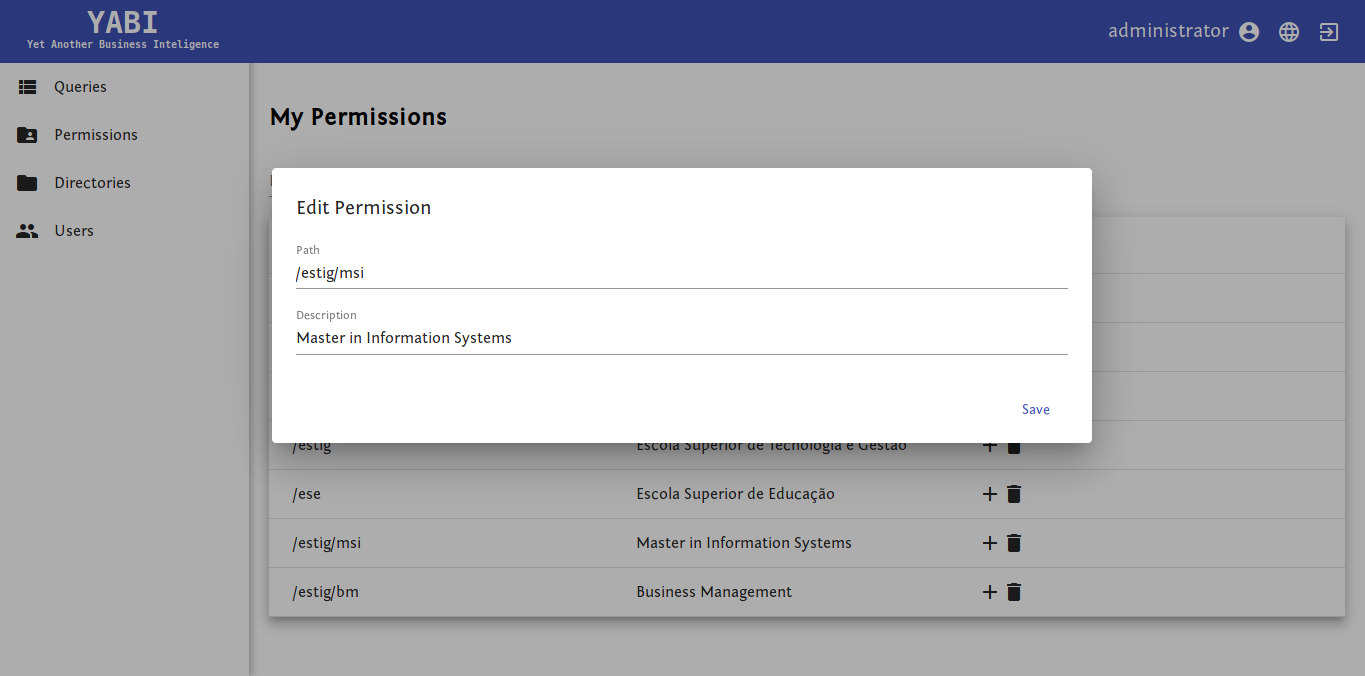
\includegraphics[width=.8\textwidth]{images/screenshots/permission/permission-edit}
  \caption{Dialog for editing an existing \texttt{Permission}}\label{fig:permissionedit}
\end{figure}


user
\begin{figure}
  \centering
  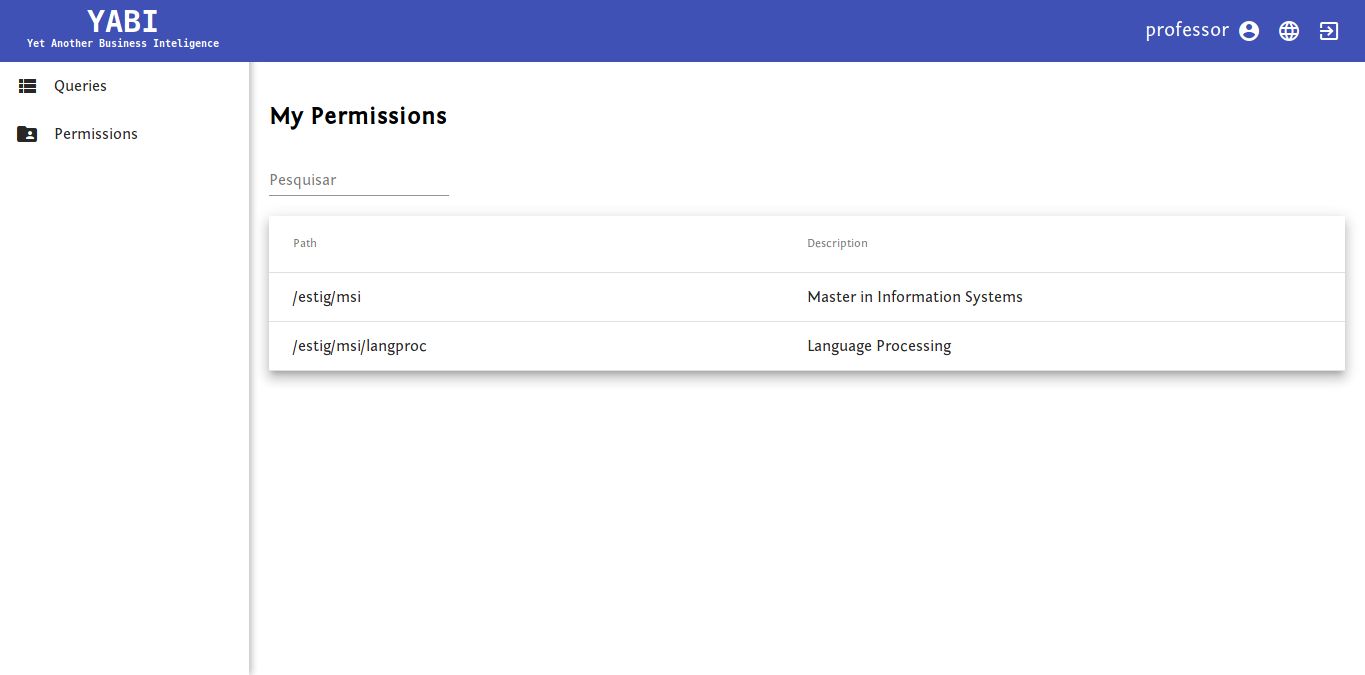
\includegraphics[width=.8\textwidth]{images/screenshots/user/user-permission-listing}
  \caption{Listing of all registered \texttt{Permission} for a given \texttt{User}}\label{fig:userpermisisonlist}
\end{figure}

\begin{figure}
  \centering
  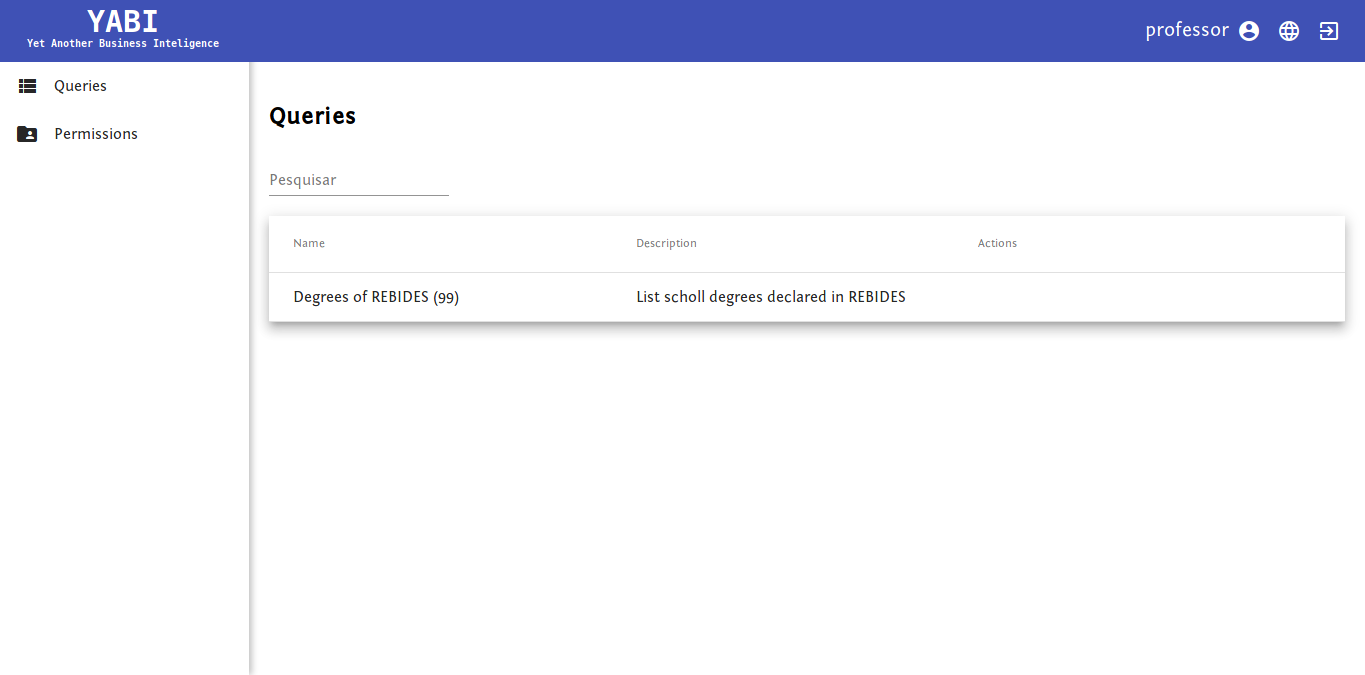
\includegraphics[width=.8\textwidth]{images/screenshots/user/user-query-listing}
  \caption{Listing of all registered \texttt{Query} for a given \texttt{User}}\label{fig:userquerylist}
\end{figure}

\begin{figure}
  \centering
  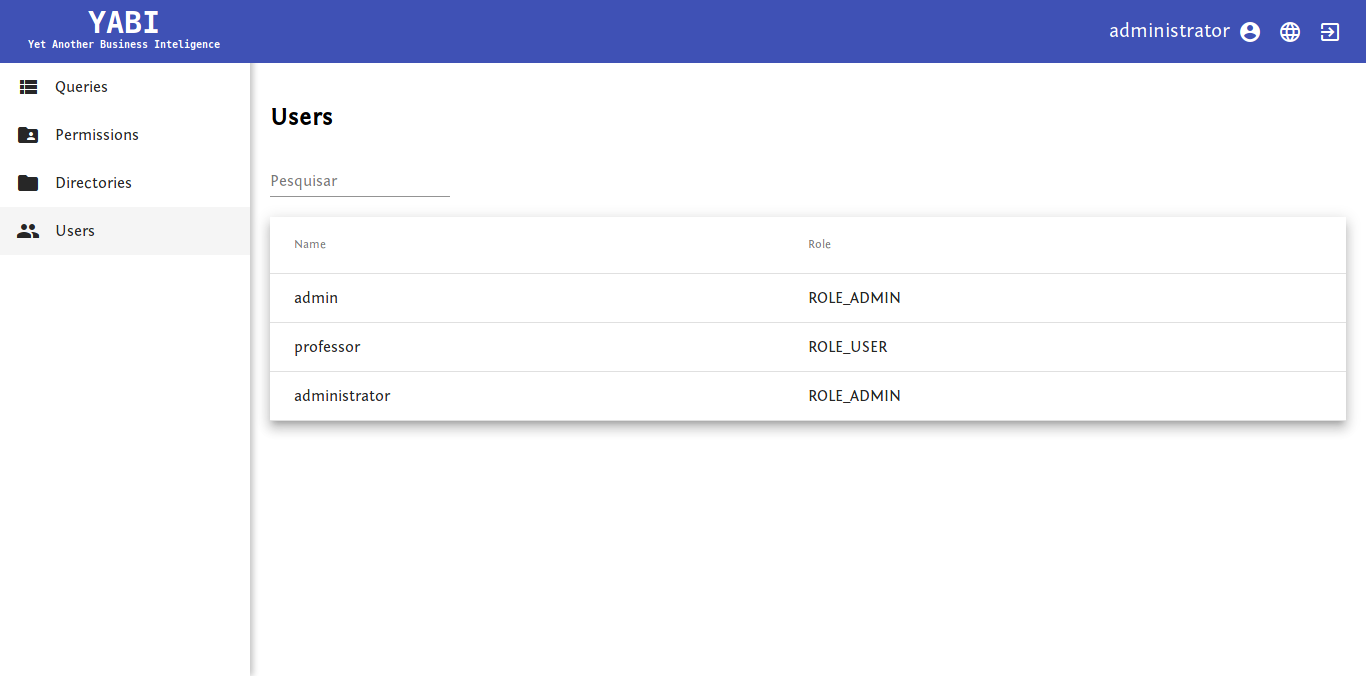
\includegraphics[width=.8\textwidth]{images/screenshots/user/user-listing}
  \caption{Listing of all registered \texttt{User}}\label{fig:userlist}
\end{figure}

\begin{figure}
  \centering
  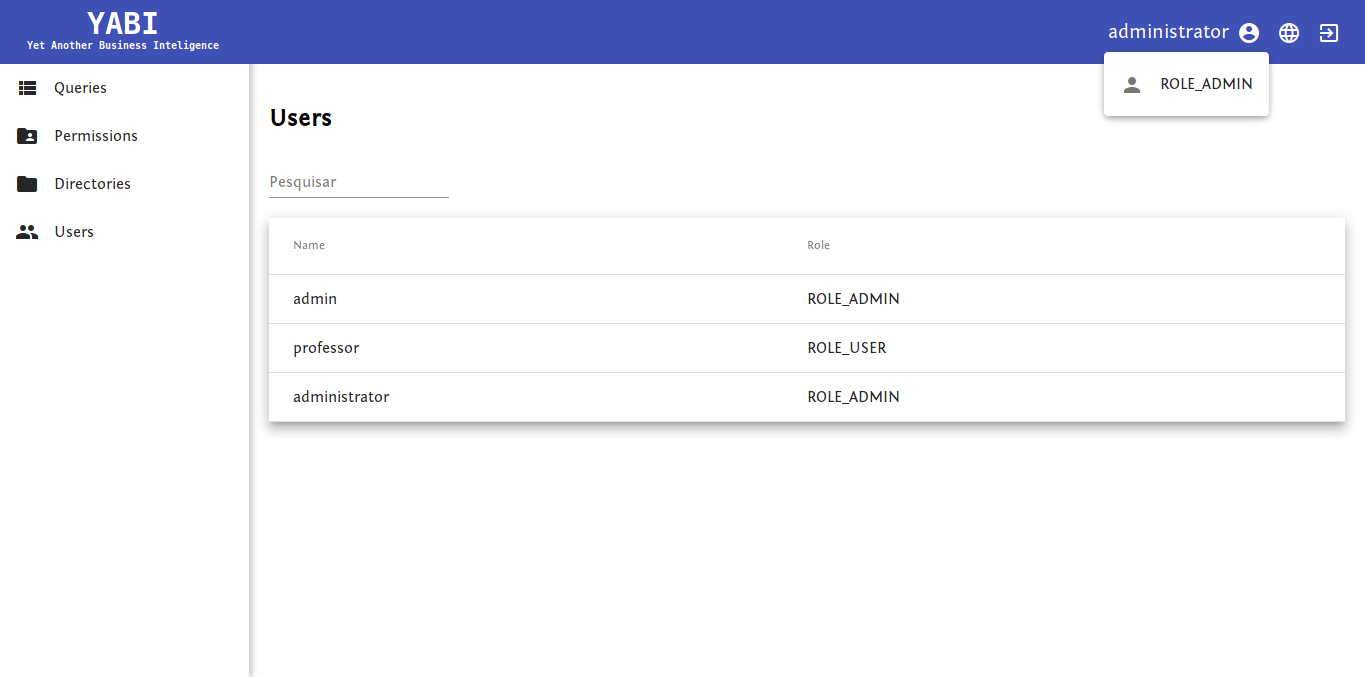
\includegraphics[width=.8\textwidth]{images/screenshots/user/admin-role}
  \caption{Small pop-up showing the current user's role}\label{fig:userrole}
\end{figure}

\begin{figure}
  \centering
  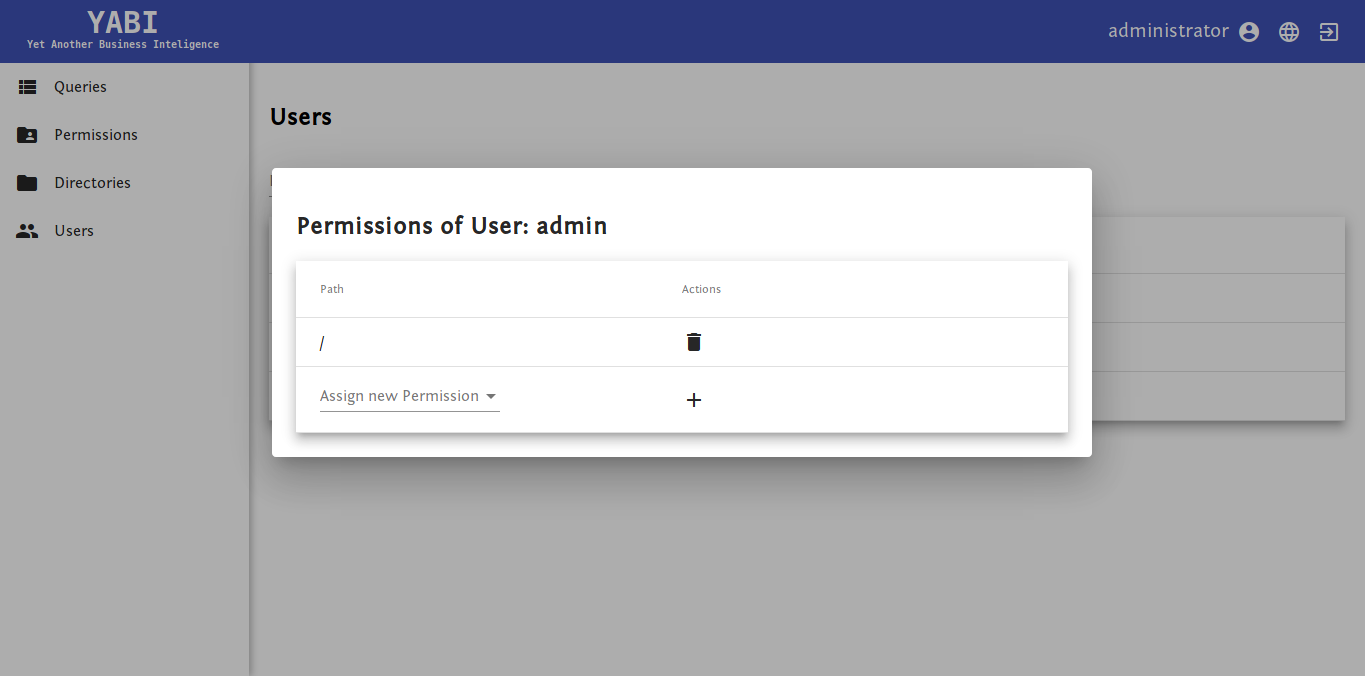
\includegraphics[width=.8\textwidth]{images/screenshots/user/admin-permission-new}
  \caption{Dialog for assigning a new \texttt{Permission} to a \texttt{User}}\label{fig:adminpermisisonnew}
\end{figure}

\subsubsection{Services}
Angular services are an abstraction over the remote \gls{API}. In this implementation, almost all resources are provided by Spring Boot's Repository interface, yielding a standard \gls{HATEOAS} reply no matter the entity. Given such repetition, it made sense to implement a common interface through which all Angular Services could inherit and extend the interaction with Spring's \texttt{PagingAndSortingRepository}.

At this point the peculiarities of each repository will be shown, implementation of the general purpose service is found in Section~\ref{hateoas:service}.

\texttt{LoginService} is concerned with providing login functionality and system-wide predicates about the current user or session. The two main predicates are \textit{isAdmin} and \textit{isAuthenticated}, the first is used on templates to hide elements that should not be seen by non-administrative users and the second is run before every request sent to \gls{API} so that the application can redirect to the login page if by some reason the user access a page without first logging-in. It also provides \textit{login} and \textit{logout}, the former saves the username and password combination in the local storage to be used by \texttt{authenticationInterceptor} and requests the \gls{API} route \textbf{/user} for information about the current user; the latter deletes the current user's instance, clears the local storage information and redirects to the login page at \textbf{/login}.

\subsubsection{Modules}
\dots
\subsection{Generic Form Control Builder}

\subsection{Spring HATEOAS Classes}
\dots
\subsubsection{Entity Class}
\dots
\subsubsection{Acessor Class}
\dots
\subsubsection{Repository Class}
\dots
\subsubsection{Repository Service Class}\label{hateoas:service}
\dots
\subsection{Temporal Caching Repository}
\dots
\subsection{Error Handler}
\dots
\subsection{Database Reader}
\dots
\subsection{authenticationInterceptor}
Because the back-end handle requests in a stateless fashion, authentication information must be sent alongside every \gls{API} request.

This was achieved by creating a class \texttt{authenticationInterceptor} that implements the \texttt{HttpInterceptor} interface, overriding the method \textit{intercept} so that requests going to the \gls{API} have a \gls{HTTP} \texttt{Authorization} header attached to it.

There are some occasions that require different or no treatment. If the request is not destined to \gls{Yabi}'s \gls{API}, the request is processed as usual and if the user is not authenticated the application redirects to \textbf{/login}, prompting the user to login again.

\subsection{apiEndpoint}
Though as a Service, this class is made available through the app's global module and can be injected into classes that declare dependency on it.

It's job is to abstract all the endpoints available in the interface either through constant strings that point to repositories or functions that assemble an address for an entity given it's id.

As an example endpoint, the \texttt{PERMISSIONS} attribute refers to the \gls{API}'s \textbf{/permissions} endpoint that return all the permissions associated to the current user; \texttt{ADMIN_PERMISSIONS} refers to \textbf{/permissionTrees}, which is the interface managed by a Spring Repository; Lastly there is the \textbf{USER_PERMISSION} function that takes in an user id and a permission id and returns the address that represents the association between them so it can be deleted.

\subsection{Shared Module}


\subsection{Security Concerns}

When a user logs-in the application, their username and password is stored as a base64 string in the local storage. Should the application be compromised with attacks such as \gls{XSS}, the injected code is able to access the user's credentials.

Another concern is in regards to the stateless nature of the back-end, requiring the credentials to be sent with every request. If the connection is not encrypted, credentials will be sent as plain base64 encoded string, which is easy to spot and decode. In the front-end this can be mitigated with \gls{HTTPS} encryption and in the general view a token could be exchanged to avoid having the credentials being frequently sent to the \gls{API}.

\section{Back-end}\label{cha:implementation:sec:back-end}
\dots

\subsection{Entities}
Following the class diagram in Figure~\ref{fig:classdiagram} and their relations, classes were created and properly annotated with so that \gls{JPA} is able to properly generate a relational model. Hence the \texttt{Entity} annotation is present in all classes.

Listing~\ref{code:sqlquery} presents the implementation of the Query model defined in Section~\ref{model:query}, it servers as an overview into other model implementations as it shares much of the common features but also adds some of its own.

Lines 1, 2 and 5 are provided by the Lombok package as discussed in Section~\ref{tech:lombok}, instructing the creation of constructor and other common methods during compilation. All models make use of \texttt{@Data} and \texttt{@NoArgsConstructor} annotations and all but \texttt{PermissionTree} uses \texttt{@AllArgsConstructor}.

In regards to \gls{ORM}, \texttt{@Entity} annotation in line 3 is the entry-point through which \gls{JPA} evaluates what classes are meant to be taken into account when building the relational model.
In general, some attributes need don't need to be declared as they are correctly inferred but in some cases it is desired to configure the generated database, \texttt{@Column} annotation on line 11 changes the default behavior so that the length of the corresponding \texttt{varchar} field in the table is able to hold larger amounts of characters; The other models, \texttt{YabiUser} \texttt{PermissionTree} and \texttt{Directory} make extensive use of \texttt{@Column} to specify columns that shouldn't have repeated values.

Relation between entities are made though \texttt{@OneToOne}, \texttt{@ManyToOne} and \texttt{@ManyToMany} annotations.
The first two represents single value association between entities, however, they represent different semantics and where the foreign key will be created.
\texttt{@ManyToOne} indicates that the foreign key will stay in the table in which this model is mapped to, \texttt{@OneToOne} makes no distinction, leaving for the \gls{ORM} back-end implementation to decide.
Line 17 is declaring that more that one instance of \texttt{SqlQuery} may reference a single \texttt{Directory} and that \texttt{SqlQuery} will hold the foreign key to \texttt{Directory}.
\texttt{@ManyToMany} represents a collection of associations, here used to associate \texttt{YabiUser} to \texttt{PermissionTree} so that many users can have many, overlapping, permissions. One possible parameter to \texttt{@ManyToMany} is the \texttt{FetchType}, instructing the \gls{ORM} engine to retrieve the associated entity only when it is accessed or together with its parent is retrieved.

\texttt{@JoinColumn} annotation is a general purpose configuration for relational fields, in line 18 and 22 it's used to configure the name in which the column will be called and whether it can have no specified value.

\lstinputlisting[firstline=22,float,
caption=Implementation of the Query model,
label=code:sqlquery
]{listings/SqlQuery/SqlQuery.java}

The remaining entities follow a similar pattern in it's implementation.

\subsection{Spring Configuration}
In order for Spring Framework to stay out of the way as much as it can and allow developers to focus on the implementation of business functionalities, it makes many assumptions about how its components interact, however, at some point the application being developed grow some needs that conflict with Spring defaults. When this eventually happens, which was the case with \gls{Yabi}, developers can override some of Spring's default behavior by implementing specific interfaces. More on Spring can be found in Section~\ref{concept:spring}.

This section presents Spring configurations that took place so that \gls{Yabi} is able to work as expected.

\subsubsection{Security}
\gls{Yabi}'s security model uses a directory server to authenticate and a relational database to load user roles and execute authorization checks. Because this is a stateless application, every request follows the steps shown in Figure~\ref{fig:authseq} before being executed by the controllers.

Authentication is done through a anonymous bind to a \gls{LDAP} server, Section~\ref{impl:ldap} goes through the Spring configuration necessary to make it work and Section~\ref{impl:detailsmapper} explains how the roles are loaded into the Sprig Security's \texttt{UserDetails} object.

In regards to authorization, there are two possible roles in which a use must be assigned to, either \texttt{ADMIN} or \texttt{USER}. With this, non-administrative resources are simply not dependent on the user's role therefore accessible to all users, meanwhile, administrative resources are explicitly marked to be accessible by users whose role is \texttt{ADMIN}, more on this in Section~\ref{impl:admres}.

Figure~\ref{fig:authseq}, presents in a general view the steps taken to authenticate and load an user's details. It is infeasible to model the whole of Spring Web and Spring Security as it is quite a extensive feature and it is out of the scope of this report, therefore it was abstracted into fewer elements, namely \texttt{WebSecurity} entity representing the objects that gets built by the configuration shown in Listing~\ref{code:authblock}, the \textit{authenticate} message is abstracting Spring's authentication provider voting system, \texttt{LDAP AuthenticationManager} entity representing \gls{LDAP}'s \texttt{AuthenticationProvider} and \textit{anonymous bind}, as the name implies is the authentication that takes place in the directory server.

The main point of Figure~\ref{fig:authseq} is to show that once the bind takes place in the \texttt{LDAP AuthenticationManager}, the library requests an object that implements the \texttt{UserDetailsContextMapper} to populate it's newly created \texttt{Authentication} object with business-specific information in the form of a \texttt{UserDetails}. In this case \texttt{YabiUserDetailsManager} is chosen by Spring's dependency injection mechanism and it provides an instance of \texttt{YabiUser}, which implements \texttt{UserDetails} interface, that is retrieved from \gls{Yabi}'s database.

\begin{figure}
  \centering
  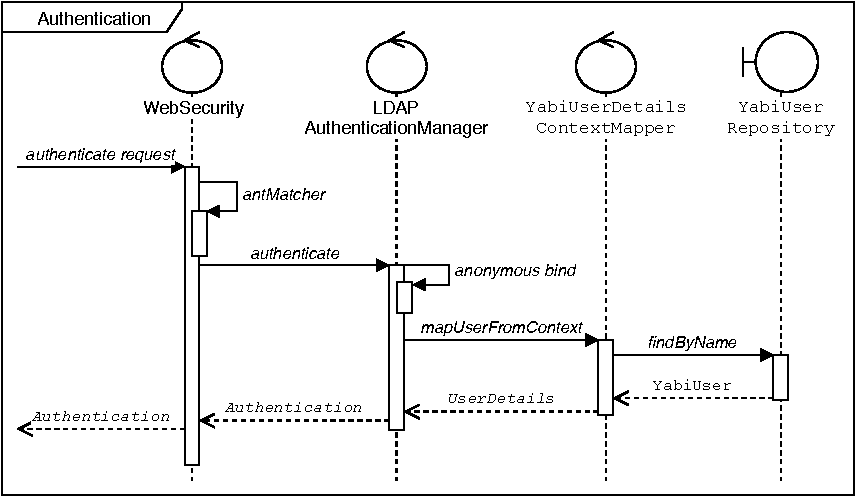
\includegraphics[width=.9\textwidth]{images/diagramas/authentication}
  \caption{Authentication Sequence Diagram}\label{fig:authseq}
\end{figure}


\subsubsection{Admin Resources}\label{impl:admres}
Not all endpoints are freely accessed to all users because they involve possibly destructive interactions with the information contained in the system. In this implementation, non-administrative users get their information through custom \texttt{RestController} that expose fewer functionalities and administrative users may directly request the repositories. Repositories are further discussed in Section~\ref{impl:repos}.

Suffice to say that certain endpoints require the user to be authenticated and to have an administrator role. Listing~\ref{code:authblock} is the configuration that enforces this statement.

The call to \texttt{antMatchers} in lines 47, 49 and 51 works by specifying a list of \gls{HTTP} paths and applying some definitions or restrictions whenever an incoming request is a member of it. \todo{membro da lista de caminhos http}. In this specific case, all requests to repositories are eligible to continue only if the \texttt{hasRole} definition evaluates to true.

Line 51 is protecting the \textbf{/permission} endpoint from being requested with a \gls{HTTP} \textsc{delete} verb.
Lines 46 and 52 declare that all \gls{HTTP} requests are to be authenticated.

\todo{as linhas estao certas ?}
\lstinputlisting[firstline=39, lastline=55, float,
caption=HttpSecurity configuration,
label=code:authblock
]{listings/Configuration/SecurityConfiguration.java}

\subsubsection{\gls{CORS} Mapping}

Because \gls{Yabi} is a web \gls{API} and a front-end application, it is necessary that both parties can interact but due to security reasons, most browsers implementations block \gls{AJAX} calls if the remote server does not explicitly add the current domain to it's response header.

In Spring, specifying allowing domains to access it's resources is done by implementing the \texttt{WebMvcConfigurer}, overriding the method \textit{addCorsMapping(CorsRegistry)} and calling \textit{allowedOrigins} on it's parameter. The method \textit{allowedOrigins} takes a list of stings that contain valid \gls{URL} addresses.

\gls{Yabi} configures this using the \texttt{application.properties} file under the key \texttt{yabi.web.allowedOrigins}, allowing for a centralized configuration.

\subsubsection{\gls{LDAP}}\label{impl:ldap}

Following the authentication specification in Section~\ref{proj:auth}, Listing~\ref{code:ldapauth} presents the configuration that implements the desired behavior.

\lstinputlisting[firstline=57, lastline=66, float,
caption=LDAP Authentication Configuration,
label=code:ldapauth
]{listings/Configuration/SecurityConfiguration.java}

\todo{checar linhas no listing gerado}
In this configuration, \texttt{AuthenticationManagerBuilder} is a class used by Spring in it's security pipeline. It comes with built-in support for \gls{LDAP}, \gls{JDBC} and in-memory authentication mechanisms; line \todo{4} is declaring \gls{LDAP} authentication to be used.

Line \todo{5} is considered important because it is mapping a custom details context mapper to the authentication pipeline. What this does is to provide a hook in the authentication pipeline to allow explicit customization of the user object after it is authenticated. The given mapper, \texttt{YabiUserDetailsContextMapper} retrieves the authenticated user's instance of \texttt{YabiUser}.

Lines \todo{6 to 9} configure the connection to the remote directory service, including it's address and what to bind with.

\subsubsection{User Details Context Mapper}\label{impl:detailsmapper}
Often times a directory service is used as an authentication mechanism. Applications issue an anonymous bind request to the server passing their user's credentials and if properly found and matched, a boolean value is returned, however, applications often has information about the user that must be sent accessible to other parts of the framework. To do so, Spring Security utilizes this interface to retrieve a \texttt{UserDetails} instance that gets injected into the commonly accessible \texttt{Authentication} interface.

For this application, a new implementation of the \texttt{UserDetailsContextMapper} interface is provided, \texttt{YabiUserDetailsContextMapper} returns an instance of \texttt{YabiUser}, which implements said \texttt{UserDetails} interface and adds \gls{Yabi}-specific attributes, enabling other parts of the system to query the current user's related information such as their role, \texttt{PermissionTree} and name. More information about the \texttt{YabiUser} class is found in Section~\ref{model:user}.

\subsection{Custom Controllers \& View Models}
\texttt{RestController} is a Spring Web annotation that enables a given class or method to handle \gls{HTTP} requests. In essence it is a combination of two other annotations, the \texttt{Controller}, which is what trigger the framework into considering the class as a possible resolver of  \gls{HTTP} requests and \texttt{ReponseBody}, that wraps the method call into a response body. In simple cases the returned Object is mapped to a \gls{JSON} string.

Because the \texttt{PermissionTree} class contains a reference to it's parent, and the root references itself, there was a need to circumvent a infinite loop during it's \gls{JSON} serialization. To do so, rather simple and 
serializable classes whose role were to convey information to the front-end were written, namely, \texttt{SqlQueryViewModel}, \texttt{PermissionTreeViewModel} and \texttt{YabiUserViewModel}.

To accommodate the special handling of \texttt{PermissionTree} model and provide some custom functionalities some custom \texttt{RestController} were implemented, \texttt{SqlQueryController}, \texttt{PermissionTreeController} \texttt{YabiUserController} and \texttt{DatabaseReaderController}.

\todo{isso esta errado, sql query é filtrado pelo metodo do controller findByPermissionNodePathStartingWith}
\todo{Filtering in relation to \texttt{Permission} was required when providing \texttt{SqlQuery} and \texttt{PermissionTree} objects to non-administrative users, it was implemented by iterating over the current user's permissions and appending all the elements under that permission to a list. Listing~\ref{code:queries} presents the implementation of such filtering applied to \texttt{SqlQuery} model.
}
\lstinputlisting[firstline=27,lastline=39, float,
caption=\textbf{/queries} Endpoint,
label=code:queries
]{listings/SqlQuery/SqlQueryController.java}

\subsubsection{DatabaseReaderController}
\todo{esta ruim}
\todo{qual eh o path que ele escuta, qual eh o argumento que ele recebe ?, como ele faz a checagem de permissao ? }
The retrieval of information contained in a remote database is exposed through the \texttt{DatabaseReaderController}. It's a wrapper to \texttt{DatabaseReader.runQuery} method that does a permission check before executing.

\subsubsection{PermissionTreeController}
Because of it's tree-like nature, once a \texttt{PremissionTree} is deleted, all of it's child nodes need also to be removed. However, because it reference its parent but not its children, leaving the \gls{RDBMS} to execute a cascading delete would delete every parent permission untill the root node.
Therefore \texttt{PermissionTreeController} implements a custom a delete that cascades through its children. It is bound to a \textsc{delete} \textbf{/pemrission/\{id\}}, \texttt{id} being the identifier of the permission to be deleted.

It is implemented by first retrieving the permission whose id was specifies in the \gls{HTTP} request, retrieve all of its children with the custom repository method \textit{findAllByNodePathStartingWith} and sequentially deleting all permissions found and lastly delete the permission itself.

One restriction is that the root node can never be deleted. Therefore, before executing the before-mentioned steps, the permission to be deleted is matched with the root node, if it does, the operation is aborted with an error.

\subsubsection{YabiUserController}
To provide the front-end with information about the current user, \texttt{YabiUserController} replies to \textsc{get} requests on the path \textbf{/user} with information contained inside the \texttt{Authentication} that was generated during the user's authentication procedure and thus avoid reaching out to the database a second time.

\subsubsection{SqlQueryController}
\texttt{SqlQuery} is one of those entities that are related to the current logged-in user. In other words, administrators may see all registered \texttt{SqlQuery} and users see only those which they can run, Therefore \texttt{SqlQueryController} was created.

It has only one method that replies to \textsc{GET} requests to \textbf{/queries} endpoint with a list of \texttt{SqlQueryViewModel}. Implementation-wise it returns a list containing every \texttt{SqlQuery} found in the database by calling \texttt{SqlQueryRepository.findAllByNodePathStartingWith} for every permission associated to the current \texttt{YabiUser}.

\subsection{Spring Repositories}\label{impl:repos}
\texttt{PagingAndSortingRepository} were created for all entities evaluated during the project evaluation phase.
The \texttt{Directory} entity whose did not require any changes in regards to what Spring already provides and won't be discussed.
The remaining entities had their repositories augmented with functionalities presented below.

\subsubsection{YabiUserRepository}
After binding in the directory service, \texttt{UserDetailsContextMapper.mapUserFromContext} is used to fill an instance of \texttt{Authentication} class with business data. In \gls{Yabi}'s custom implementation, this data comes from a relational database that reflect \texttt{YabiUser} objects.

Because the method \textit{mapUserFromContext} uses the username as a key to retrieve information, \texttt{YabiUserRepository} had to be augmented with a new method to do just that. Therefore the following declaration was added:\\
\texttt{YabiUser findByName(String username);}

\subsubsection{PermissionTreeRepository}
When the system needs to validate an action or filter information depending on a permission, it retrieves all of its child permissions. Because this action is frequently used, this repository had also to be augmented.

In this case, the method signature used was as follows:\\
\texttt{List<PermissionTree> findAllByNodePathStartingWith(String~nodePath);}

\subsubsection{SqlQueryRepository}
When an user request a list of queries that they can execute, the system must retrieve from the relational database all queries in which the permission is a child of the user's permission. Again, this repository had to be augmented.

This was accomplished by using the following method interface:\\
\texttt{List<SqlQuery> findByPermissionNodePathStartingWith( String~nodePath );}

\subsection{Multi-Database Support}
Paraphrasing Requirement~\ref{req:multidb}, the application must be able to retrieve information from the institution's database. However, because it has many in-house applications, they might use different \gls{RDBMS} and \gls{Yabi} should then be able to connect to then.

The core part of this feature is \gls{JDBC} 4.0's \texttt{DriverManager} class and it's \textit{getConnection} method that upon being called, attempts to make a connection using drivers that were loaded on initialization-time, therefore, as long as the driver is loaded and the connection string is properly formed, \textit{getConnection} will select the correct database driver.

Because of this, implementing this feature was as simple as declaring dependencies for database drivers in the \texttt{pom.xml} configuration file. Notably, Oracle\footnote{https://www.oracle.com/technetwork/database/database-technologies/express-edition/downloads/index.html} requires the creatin of an Oracle account and configuring a custom maven repository in order to download their drivers.

\section{Development Environment}\label{cha:implementation:sec:development}
This section will focus on the tools that were configured to accommodate the development and testing of this application.

\subsection{Directory Service}
When developing an application, it is good practice to avoid reaching out and interacting to remote services and instead provide a local instance that is able to mimic the real-world one.

In this case because a directory service is used as a part of it's authentication mechanism, a local \gls{LDAP} server was created in Apache Directory Studio that mimics \gls{IPB}'s directory service enough so that the configuration provided by their \gls{IT} team is able to be used locally with minimal changes, in fact, the only difference is the service's address.

Listing~\ref{code:ldapconfig} exposes the configurations \gls{Yabi} uses to access the server, note that the directory address is declared in line 1 and line 3 declare the entry whose elements are anonymously bound.

\lstinputlisting[firstline=13,lastline=15, float,
caption=Local server \gls{LDAP} configuration,
label=code:ldapconfig
]{backendlink/src/main/resources/application.properties}

Figure~\ref{fig:adsconfig} show how the directory is structured in the server-side. Users are of class \texttt{inetOrgPerson}, they are held under the \texttt{users} organizational unit which in turn is under the \texttt{ipb}, \texttt{pt} domain component. At the moment this figure was taken, passwords were stored in plain text for local testing purposes.

\begin{figure}
  \centering
  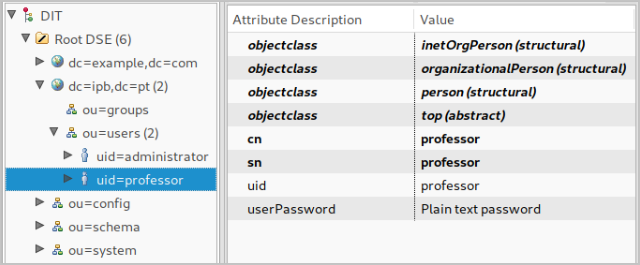
\includegraphics[width=.8\textwidth]{images/screenshots/ldap-directory}
  \caption{Directory structure and the properties of user \texttt{professor}}\label{fig:adsconfig}
\end{figure}

\subsection{Database Initializer}
When starting \gls{Yabi} for the first time, it needs to generate its database, create the root permission and an administrator account.
To do so, the class \texttt{DbInitializer} was written. It implements the \texttt{CommandLineRunner} interface so that Spring instantiate and runs it upon initialization.

There are two properties that interact with \texttt{DbInitializer}, \texttt{yabi.db.init} and \texttt{yabi.db.init.admin.username}. The former regulates when yabi should create a new database, the root permission and the administrator account, the latter declares the administrator's username that should be used. If the initialization is desired, \texttt{yabi.db.init} should be set to \texttt{create}, otherwise, it should be set to anything else. It is necessary that the administrator username is able to be bound in the directory service otherwise the authentication will fail.

\subsection{Postman Tests}
When developing the \gls{API}, some test cases were created in Postman to assess the prevention of data duplication. All four entities were tested.
In essence, every test consists of two requests, one that creates a new entity and expects a \gls{HTTP} status 201 response and the other that tries to re-create the same entity and expects a \gls{HTTP} status 409.

It is important to note that these tests are validating the following restrictions imposed in each entity:
\begin{itemize}
\item There must be only one \texttt{PermissionTree} per \texttt{nodePath}.
\item One \texttt{Directory} per \texttt{connectionString} so that each database is referenced once.
\item One \texttt{Directory} per \texttt{name} so that each name maps to only one database.
\item One \texttt{SqlQuery} under a \texttt{PermissionTree} with a given \texttt{name}, avoiding ambiguous \texttt{SqlQuery} entries.
\item No more than one \texttt{YabiUser} with a given \texttt{name}.
\end{itemize}

\subsection{Conclusion}
This section discussed the implementation details all the parts that compose the \gls{Yabi} application and its development.
\todo{Bruno! o que colocar na coclusao ?}



